\documentclass[a4paper, 10pt]{paper}
\usepackage{graphicx}
\usepackage{fullpage}
\usepackage{amsmath}
\usepackage{amssymb}
\usepackage{hyperref}
\usepackage{tcolorbox}
\usepackage{tikz}
%\usepackage{MnSymbol}

\newcommand{\be}{\begin{eqnarray*}}
\newcommand{\ee}{\end{eqnarray*}}
\newcommand{\beq}{\begin{eqnarray}}
\newcommand{\eeq}{\end{eqnarray}}
\newcommand{\bk}{{\mathbf{k}}}
\newcommand{\bK}{{\mathbf{K}}}
\newcommand{\bp}{{\mathbf{p}}}
\newcommand{\bq}{{\mathbf{q}}}
\newcommand{\bm}{{\mathbf{m}}}
\newcommand{\br}{{\mathbf{r}}}
\newcommand{\bu}{{\mathbf{u}}}
\newcommand{\bR}{{\mathbf{R}}}
\newcommand{\bS}{{\mathbf{S}}}
\newcommand{\ba}{{\mathbf{a}}}
\newcommand{\bb}{{\mathbf{b}}}
\newcommand{\bc}{{\mathbf{c}}}
\newcommand{\bd}{{\mathbf{d}}}
\newcommand{\bbe}{{\mathbf{e}}}
\newcommand{\bB}{{\mathbf{B}}}
\newcommand{\bA}{{\mathbf{A}}}
\newcommand{\bE}{{\mathbf{E}}}
\newcommand{\bF}{{\mathbf{F}}}
\newcommand{\bJ}{{\mathbf{J}}}
\newcommand{\bP}{{\mathbf{P}}}
\newcommand{\bX}{{\mathbf{X}}}
\newcommand{\bv}{{\mathbf{v}}}
\newcommand{\bs}{{\mathbf{s}}}
\newcommand{\bfe}{{\mathbf{e}}}
\newcommand{\bt}{{\mathbf{t}}}
\newcommand{\bg}{{\mathbf{g}}}
\newcommand{\dd}{\mathrm{d}}
\newcommand{\bhx}{\hat{\mathbf{x}}}
\newcommand{\bhy}{\hat{\mathbf{y}}}
\newcommand{\bhz}{\hat{\mathbf{z}}}
\newcommand{\bhw}{\hat{\mathbf{w}}}
\newcommand{\bx}{{{\mathbf{x}}}}
\newcommand{\by}{{{\mathbf{y}}}}
\newcommand{\h}{\hat{H}}
\newcommand{\hp}{\hat{P}}
\newcommand{\up}{\uparrow}
\newcommand{\down}{\downarrow}
\newcommand{\ph}{{\phantom{\dagger}}}
\newcommand{\ket}[1]{\left|{#1}\right\rangle}
\newcommand{\bra}[1]{\left\langle{#1}\right|}
\newcommand{\hc}{\mathrm{H.c.}}
\newcommand{\ado}{a^\dagger}
\newcommand{\bdo}{b^\dagger}
\newcommand{\ddp}{\partial}

\newcommand{\mcA}{\mathcal{A}}
\newcommand{\mcB}{\mathcal{B}}
\newcommand{\mcC}{\mathcal{C}}
\newcommand{\mcD}{\mathcal{D}}
\newcommand{\mcM}{\mathcal{M}}
\newcommand{\mcN}{\mathcal{N}}

\newcommand{\bn}{\mathbf{n}}
\newcommand{\id}{\mathbb{I}}
\newcommand{\zbb}{\mathbb{Z}}
\newcommand{\zb}{\bar{z}}

\newcommand{\tr}{\mathrm{tr}}
\newcommand{\Tr}{\mathrm{Tr}}

\newcommand{\kb}[2]{\ket{#1}\!\bra{#2}}
\newcommand{\kbd}[2]{\ket{#2}\!\bra{#1}}

\newcommand{\ketx}[1]{\left|{\frac{\partial^{#1}\tilde{u}_n}{\partial {k_x}^{#1}}}\right\rangle}
\newcommand{\brax}[1]{\left\langle{\frac{\partial^{#1}\tilde{u}_n}{\partial {k_x}^{#1}}}\right|}
\newcommand{\kety}[1]{\left|{\frac{\partial^{#1}\tilde{u}_n}{\partial {k_y}^{#1}}}\right\rangle}
\newcommand{\bray}[1]{\left\langle{\frac{\partial^{#1}\tilde{u}_n}{\partial {k_y}^{#1}}}\right|}

\newcommand{\keto}{\ket{\tilde{u}_n}}
\newcommand{\brao}{\bra{\tilde{u}_n}}

\newcommand{\ketxy}[2]{{\left|\frac{\partial^{#1+#2}\tilde{u}_n}{\partial {k_x}^{#1}\partial {k_y}^{#2}}\right\rangle}}
\newcommand{\braxy}[2]{\left\langle{\frac{\partial^{#1+#2}\tilde{u}_n}{\partial {k_x}^{#1}\partial {k_y}^{#2}}}\right|}

\newcommand{\bbn}{\bra{\tilde{n}}}
\newcommand{\bkn}{\ket{\tilde{n}}}
\newcommand{\bbm}{\bra{\tilde{m}}}
\newcommand{\bkm}{\ket{\tilde{m}}}

\newcommand{\kx}{\hat{k}_x}
\newcommand{\ky}{\hat{k}_y}

\begin{document}
\title{Quartic Hamiltonians in the Hofstadter Model}
\maketitle
%%%%%%
In this document, we obtain the Hofstadter model hopping amplitudes that lead to quartic Hamiltonians.
%%%%
\section{Hopping Terms on the Square Lattice}
We first consider a tight-binding model on a square lattice which involves hops between each site and its three sets of nearest neighbours. We write the (assumed real) hopping amplitude to each set of neighbours as $t_1$, $t_2$ and $t_3$, respectively, as shown below:
\begin{center}
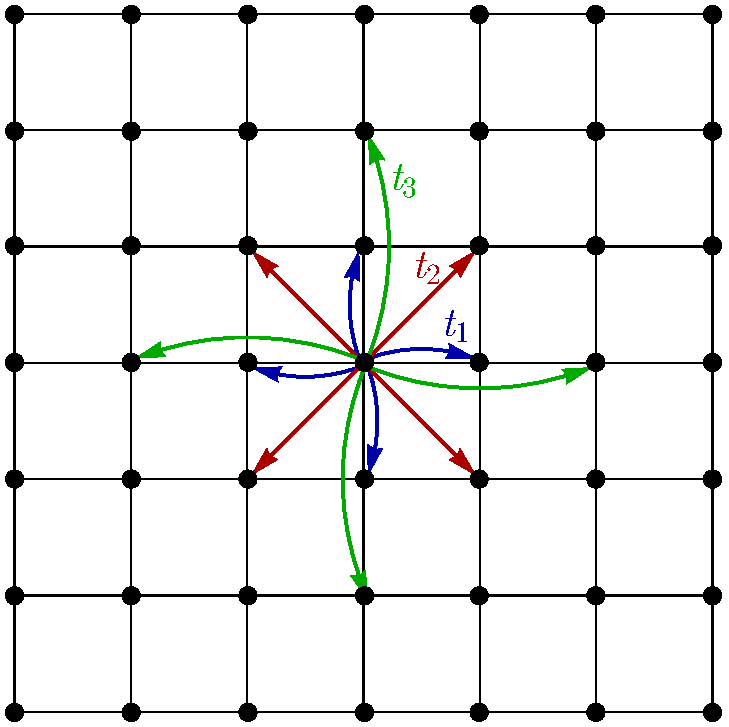
\includegraphics[scale=0.5]{hoppingterms.pdf}
\end{center}
In the absence of a magnetic field, the corresponding tight-binding model can be written
\be
\h&=&\sum_{\br}\bigg[t_1\left(c^\dagger_{\br+\bhx}c^\ph_{\br}+c^\dagger_{\br-\bhx}c^\ph_{\br}+c^\dagger_{\br+\bhy}c^\ph_{\br}+c^\dagger_{\br-\bhy}c^\ph_{\br}\right)\\
&&+t_2\left(c^\dagger_{\br+\bhx+\bhy}c^\ph_{\br}+c^\dagger_{\br-\bhx+\bhy}c^\ph_{\br}+c^\dagger_{\br+\bhx-\bhy}c^\ph_{\br}+c^\dagger_{\br-\bhx-\bhy}c^\ph_{\br}\right)\\
&&+t_3\left(c^\dagger_{\br+2\bhx}c^\ph_{\br}+c^\dagger_{\br-2\bhx}c^\ph_{\br}+c^\dagger_{\br+2\bhy}c^\ph_{\br}+c^\dagger_{\br-2\bhy}c^\ph_{\br}\right)\bigg],
\ee
which may be diagonalised in momentum space to give
\begin{equation}
\h=\sum_{\bk}\bigg[2t_1\left[\cos(k_x)+\cos(k_y)\right]+2t_2\left[\cos(k_x+k_y)+\cos(k_x-k_y)\right]+2t_3\left[\cos(2k_x)+\cos(2k_y)\right]\bigg]c^\dagger_\bk c^\ph_\bk.\label{eq:ham}
\end{equation}
To obtain the corresponding Hofstadter Hamiltonian in the presence of a magnetic field, we should replace $\bk$ with its magnetic operator through
\be
\bk&\to&-i\nabla-\bA,
\ee
(see EM Response draft). 
%%%%
\section{Quartic Hamiltonians}
To obtain a quartic Hamiltonian, we expand Eq.~\eqref{eq:ham} order by order in momentum, finding
\be
\h(\bk)&=&4\left(t_1+t_2+t_3\right)-\left(k_x^2+k_y^2\right)\left(t_1+2t_2+4t_3\right)\\
&&+\frac{1}{12}\bigg[k_x^4\left(t_1+2(t_2+8t_3)\right)+k_y^4\left(t_1+2(t_2+8t_3)\right)+12t_2k_x^2k_y^2\bigg]+\ldots
\ee
Then, we set
\be
t_1&=&-2t_2-4t_3
\ee
to eliminate the quadratic piece, leaving
\be
\h_{O(k^4)}(\bk)&=&-4\left(t_2+3t_3\right)+t_3\left[k_x^4+k_y^4\right]+t_2k_x^2k_y^2+\ldots
\ee
In this way, we can obtain any quartic Hamiltonian we like by tuning $t_2$ and $t_3$.
\subsubsection*{Specific Parameter Choices}
In particular, if we choose
\be
t_2&=&0\\
t_1&=&-4t_3
\ee
we obtain the quartic Hamiltonian with no mixed terms,
\be
\h_{4,4}&=&-12t_3+t_3\left[k_x^4+k_y^4\right]+\ldots
\ee
On the other hand, if we choose
\be
t_3&=&0\\
t_1&=&-2t_2
\ee
we obtain the quartic Hamiltonian with only mixed terms
\be
\h_{2\times2}&=&-4t_2+t_2k_x^2k_y^2+\ldots
\ee
In all cases, we can obtain the corresponding Hofstadter Hamiltonian by replacing $\bk$ with the magnetic momentum operator.
%%%%
\section{Ladder Operator Expressions}
We rewrite some of the above expressions in terms of ladder operators by using the operator replacements
\be
\hat{k}_x&\to&-\sqrt{\frac{B}{2}}\left(a+a^\dagger\right)\\
\hat{k}_y&\to&-i\sqrt{\frac{B}{2}}\left(a-a^\dagger\right)
\ee
and being sure to replace momentum products with their fully symmetrised form.

Substituting into the expression above, we find
\be
\h_{O(k^4)}(\bk)&\to&-4\left(t_2+3t_3\right)+t_3\left[\hat{k}_x^4+\hat{k}_y^4\right]+t_2\left\{\hat{k}_x^2\hat{k}_y^2\right\}+\ldots\\
&=&-4\left(t_2+3t_3\right)+t_3\left[6 {B}^2 a^\dagger  a+3 {B}^2 \left(a^\dagger\right) ^2 a^2+\frac{1}{2} a^4 {B}^2+\frac{1}{2} \left(a^\dagger\right) ^4 {B}^2+\frac{3 {B}^2}{2}\right]\\
&&+t_2\left[{B}^2 a^\dagger  a+\frac{1}{2} {B}^2 \left(a^\dagger\right) ^2 a^2-\frac{1}{4} a^4 {B}^2-\frac{1}{4} \left(a^\dagger \right)^4 {B}^2+\frac{{B}^2}{4}\right]+\ldots\\
&=&-4\left(t_2+3t_3\right)+\frac{B^2}{4}\bigg[\left(-t_2+2t_3\right)\left(\left(a^\dagger\right) ^4+a^4\right)+2\left(t_2+6t_3\right)\left(1+2a^\dagger a + \left(a^\dagger\right)^2a^2\right)+\ldots
\ee
In particular, if we set 
\be
t_2+6t_3&=&0,
\ee
we obtain
\be
\h_{a^4,a^{\dagger4}}&=&12t_3+2B^2t_3\left(\left(a^\dagger\right) ^4+a^4\right)+\ldots,
\ee
which has no diagonal ladder operator terms.

Does this correspond to a realistic band structure? Substituting this new value of $t_2$ into the zero-field Hamiltonian, we find
\be
\h_{O(k^4)}(\bk)&=&12t_3+t_3\left(k_x^4+k_y^4\right)-6t_3k_x^2k_y^2+\ldots
\ee
In this way, the $\bk=0$ point (which we implicitly expand about) is still a band extremum (although it will not be a global extremum). In this way, I think it still makes sense to consider $\h_{a^4,a^{\dagger4}}$ as the approximate Hamiltonian in the weak-field limit for states at this point. The overall energy offset can be tuned to zero by applying an on-site energy, in which case the leading term in the Hamiltonian may be written
\be
\tilde{H}_{a^4,a^{\dagger4}}&=&2B^2t_3\left(\left(a^\dagger\right) ^4+a^4\right)
\ee

A brief play around in Mathematica suggests that this Hamiltonian has eigenstates which are very close to the quantum Harmonic oscillator states---expect that there is now a positive energy branch and a negative energy branch (each scaling as $n^2$). There are four degenerate zero-energy states fairly similar ($>90\%$) to $\ket{0}$, $\ket{1}$, $\ket{2}$ and $\ket{3}$. The positive and negative energy states with the same energy magnitude have the same density but differ by some signs (in the LL basis). Overall, I don't think the situation is very different from the case where there are $a^\dagger a$ terms (etc.) present...



\end{document}